	\documentclass[10pt,oneside]{CBFT_book}
	% Algunos paquetes
	\usepackage{amssymb}
	\usepackage{amsmath}
	\usepackage{graphicx}
% 	\usepackage{libertine}
% 	\usepackage[bold-style=TeX]{unicode-math}
	\usepackage{lipsum}

	\usepackage{natbib}
	\setcitestyle{square}

	\usepackage{polyglossia}
	\setdefaultlanguage{spanish}


	\usepackage{CBFT.estilo} % Cargo la hoja de estilo

	% Tipografías
	% \setromanfont[Mapping=tex-text]{Linux Libertine O}
	% \setsansfont[Mapping=tex-text]{DejaVu Sans}
	% \setmonofont[Mapping=tex-text]{DejaVu Sans Mono}

	%===================================================================
	%	DOCUMENTO PROPIAMENTE DICHO
	%===================================================================

\begin{document}

% =================================================================================================
\chapter{Medios materiales}
% =================================================================================================

% % =================================================================================================
% \section{Medios materiales}
% % =================================================================================================

Digamos, un poco {\it sketchi} que los medios se pueden agrupar, según sus propiedades
según el siguiente esquema.

\begin{itemize}
 \item Dieléctricos
 \item Medios magnéticos
	$\begin{cases}
	 \text{imán inducido}
		\begin{cases}
		\text{paramagnético} \\
		\text{diamagnético}
		\end{cases} \\
	 \text{imán permanente} \quad \text{ferromagnético}
	\end{cases}$
 \item Conductor
	$\begin{cases}
	 \text{perfecto} \\
	 \text{buen conductor} \\
	 \text{mal conductor}
	\end{cases}$
\item Plasmas (gas ionizado)
\end{itemize}

Podemos hacer una suerte de tabla comparativa entre eléctrico y magnético
(pero lo armaremos después con minipage)

\section{Campos estáticos en medios materiales}

\notamargen{Esta subsección tal vez mejor sería que fuera llamada
``polarización eléctrica''.}

En la picture de acá abajo tenemos un átomo esféricamente simétrico, un medio y un vector
de polarización. Entonces vemos en la vista zoom cómo se induce un dipolo

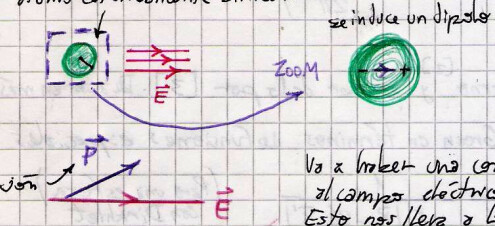
\includegraphics[width=0.6\textwidth]{images/fig_ft1_medios_campos_estaticos.jpg}

Habrá una componente dipolar paralela al campo eléctrico externo.
Esto nos lleva a la constante dieléctrica del medio (dependerá decrecientemente 
de la temperatura).

Supondremos que las propiedades macroscópicas para dos campos se satisfacen para los
campos vistos microscópicamente
\[
	\vb{\mathcal{E}}(\vbx) \to \rotorm{\mathcal{E}} = 0
\]
El campo macro \vb{E} será un promedio estadístico de su versión microscópica
\[
	\vb{E}(\vbx) = \langle \vb{\mathcal{E}}(\vbx)  \rangle =
	\frac{1}{\Delta V} \int_V \vb{\mathcal{E}}( \vbx + \vb{\chi} ) \: d^3\chi,
\]
donde $\chi$ es una coordenada que barre el volumencillo $\Delta V$.
Como vale la linealidad, se tiene $ \rotorm{\mathcal{E}} = 0 $ que conduce a
$ \rotorm{ E } = 0 $ de manera que $ \vb{E} = - \nabla \phi(\vbx) $.
El vector \vb{D} no cumple esto último.

Se construye así
\[
	\vb{P}(\vbx) = \sum_i \: N_i \langle p_i \rangle,
\]
donde la polarización  
\[
	\vb{P} = \frac{\delta \vb{p}}{\delta V}
\]
es el momento dipolar eléctrico por unidad de volumen. 

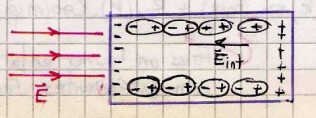
\includegraphics[width=0.45\textwidth]{images/fig_ft1_medios_picturete.jpg}	

Luego, un {\it cacho} de potencial $ \phi $ será
\[
	\delta \phi(\vbx,\vbx') = \frac{\rho_L(\vbx')}{|\vbx - \vbx'|} \delta V' +
	\vb{P}(\vbx')\cdot\frac{(\vbx - \vbx')}{|\vbx - \vbx'|^3} \delta V'
\]
de manera que el potencial
\[
	\phi(\vbx) = \int \delta \phi(\vbx,\vbx') \: d^3x' =
	\int \frac{\rho_L(\vbx')}{|\vbx - \vbx'|} \: dV' +
	\int \vb{P}(\vbx')\cdot\frac{(\vbx - \vbx')}{|\vbx - \vbx'|^3} \: dV'
\]

Ahora el último término se puede escribir como
\[
	\int_V \frac{\vb{P}(\vbx')\cdot ( \vbx - \vbx')}{|\vb{x}-\vb{x}'|^3} dV' =
	-\int_V \vb{P}(\vbx')\cdot \Nabla\left( \frac{ 1 }{ |\vb{x}-\vb{x}'| } \right) dV' 
\]
y considerando integración por partes en esta última 
\notamargen{Hay que hacer partes con sumo detalle aquí y justificar que el surface term
se arroja a los chanchos.}
\[
	\int_{V'} \frac{\rho_L(\vbx')}{|\vb{x}-\vb{x}'|} \: dV' -
	\int_{V'} \frac{ \divem{P} }{|\vb{x}-\vb{x}'|} \: dV' 
\]
que se pueden consolidar en
\[
	\phi(\vbx ) = \int_{V'} \frac{1}{|\vb{x}-\vb{x}'|}
	\left[ \: \rho_L(\vbx') - \divem{P}(\vbx') \:\right] \: dV',
\]
donde el volumen $V'$ abarca todas las fuentes (incluso las de polarización). Entonces
considerando que
\[
	\divem{P} = -\rho_P,
\]
se puede definir una densidad de carga total 
\[
	\rho_T = \rho_L + \rho_P.
\]
Entonces, el potencial se escribe como
\[
	\phi(\vbx ) = \int_{V'} \frac{\rho_T}{|\vb{x}-\vb{x}'|} \: dV'.
\]

De esta forma se puede construir un vector $\vb{D}$ siguiendo
esta línea de razonamiento:
\[
	\begin{cases}
	\rotorm{E}  = 0 \\
	\divem{E} = 4\pi\rho_T = 4 \pi ( \rho_L + \rho_P )
	\end{cases}
\]
y pasando de miembros
\[
	\divem{E} -  4 \pi \rho_P = 4 \pi \rho_L 
\]
\[
	\divem{E} + 4 \pi \divem{P} = \Nabla\cdot(\vb{E} + 4\pi\vb{P} )
\]
de modo que
\[
	\vb{D} \equiv \vb{E} + 4 \pi \vb{P} \qquad \qquad \divem{D} = 4\pi\rho_L
\]
donde \vb{D} es el llamado vector desplazamiento y estas expresiones valen para todo medio.

En la situación depicted en la figurilla siguiente

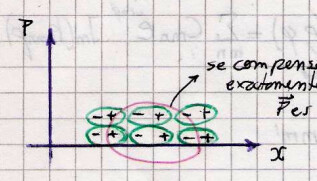
\includegraphics[width=0.4\textwidth]{images/fig_ft1_rhoP_nocompensada.jpg}

se tendrá una compensación exacta si \vb{P} es uniforme, de manera que $\divem{P}=0$. En caso
contrario existirá una $\rho_P$ no nula en el interior.

{\bf escrachos}

\notamargen{No sé qué pasaba con la parte de la integral de superficie.}
% Cuando se construye el potencial llegamos a 
% \[
% 	\int_V \frac{\vb{P}\cdot ( \vbx - \vbx')}{|\vb{x}-\vb{x}'|^3} dV =
% 	\int_V \vb{P}\cdot \frac{ 1 }{ |\vb{x}-\vb{x}'| } dV 
% \]
% y esta integral por partes lleva a lo de más abajo.


Luego el potencial es, posteriormente a haber hecho partes
es
\[
	\phi( \vb{x}) = \int_S \frac{\vb{P}(\vb{x}')}{|\vb{x}-\vb{x}'|} d\vb{S}' - 
	\int_V \frac{\Nabla\cdot\vb{P}(\vb{x}')}{|\vb{x}-\vb{x}'|}  dV'
\]
\[
	\qquad \vb{P}\cdot\hat{n} = \sigma_P \qquad \Rightarrow \qquad \divem{P} = -\rho_0
\]

Por la linealidad
\[
	\vb{P} = \xi_e \vb{E} \qquad \text{MLIH}
\]
\[
	\vb{D} = ( 1 + 4\pi\xi_e ) \vb{E} 
\]
\[
	\vb{D} = \epsilon \vb{E}
\]
donde $\xi_e$ es la susceptibilidad eléctrica y $\epsilon$ es la permitividad eléctrica.
Los contornos entre medios se resuelven según
\[
	\hat{n} \times (\vb{E}_2 -\vb{E}_1) = 0 \qquad 
	(\vb{D}_2 -\vb{D}_1)\cdot\hat{n} = 4 \pi \sigma_L \qquad 
	(\vb{P}_2 -\vb{P}_1)\cdot\hat{n} = - \sigma_P,
\]
que provienen del rotor de \vb{E}, la divergencia de \vb{D} y la divergencia
de \vb{P} respectivamente.

\subsection{Magnetismo en la materia}
\notamargen{Esta sección fue antes ``imanes inducidos''.}

Los dipolos magnéticos inducidos son de dirección opuesta al campo externo $\vb{B}$ 
(diamagnetismo).
Aquellas sustancias con momento magnético permanente se orientan en la dirección del
campo \vb{B} (paramagnético).

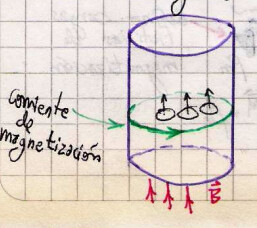
\includegraphics[width=0.4\textwidth]{images/fig_ft1_imaninducidos.jpg}

Microscópicamente se tiene un campo $\vb{b}$ que verifica $\divem{b}=0$ de manera 
que el campo total será un promedio en la región, i.e.
\[
	\vb{B} = \langle \vb{b} \rangle = 
	\frac{1}{\Delta V} \int_{\Delta V} \: \vb{b} \: (\vbx + \vb{\xi} ) \: d^3\xi,
\]
donde $\Delta V$ es microscópicamente grande pero macroscópicamente chico.
La linealidad permite que la divergencia de \vb{B} sea nula de modo que existe \vb{A}
tal que su rotor es \vb{B}.
Entonces,
\[
	\vb{M}(\vbx) = \sum_i N_i(\vbx_i) \langle \vb{m}_i \rangle
\]
donde $N_i$ es un tipo de moléculas y $ \langle \vb{m}_i \rangle$ es un momento magnético
medio. La sumatoria vale para ciertos tipos de moléculas [¿?].

Por otro lado la magnetización se puede interpretar/definir como
\[
	\vb{M} = \frac{\delta \vb{m}}{\delta V},
\]
que es el momento dipolar magnético por unidad de volumen. Luego el potencial 
\[
	\delta\vb{A} = \frac{ \delta \vb{m} \times ( \vbx - \vbx') }{|\vbx - \vbx'|}
\]
se evalúa con la misma idea que la del dipolo para polarización.
Queda por incorporar el asuntete de 
\[
	\frac{1}{c} \int_V c \vb{M} \times \Nabla\frac{ 1 }{|\vb{x}-\vb{x}'|}  dV'
	= \frac{1}{c} \int_V \frac{ c(\rotorm{M}) }{|\vb{x}-\vb{x}'|}  dV'
\]
usando partes.

\notamargen{Tenía este figurín por allí. Sería bueno ver si es una
idea importante.
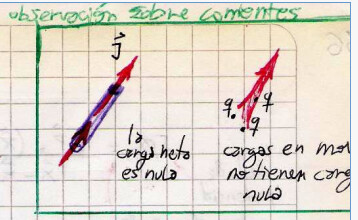
\includegraphics[width=0.375\textwidth]{images/fig_ft1_imaninducidos_nota.jpg}
}

El potencial vector puede escribirse como
\[
	\vb{A}( \vb{x}) = \frac{1}{c} \int_V 
	\left[ \frac{ \vb{J}_L(\vb{x}') }{|\vb{x}-\vb{x}'|} +
	\frac{ c \vb{M} \times (\vb{x}-\vb{x}') }{|\vb{x}-\vb{x}'|^3} \right] dV',
\]
y con el trick usual la segunda integral se convierte a 
\[
	\vb{A}( \vb{x}) = \frac{1}{c} \int_V 
	\left[ \frac{ \vb{J}_L(\vb{x}') }{|\vb{x}-\vb{x}'|} +
	\frac{ c \divem{M} }{|\vb{x}-\vb{x}'|} \right] dV'
\]
mientras que con la definición de las corrientes total y de magnetización es
\[
	\vb{A}( \vb{x}) = \frac{1}{c} \int_V 
	\frac{ \vb{J}_L(\vb{x}') + \vb{J}_M(\vb{x}' ) }{|\vb{x}-\vb{x}'|} dV'
\]
que vale para toda región donde haya corrientes libres (o desplazamientos
microscópicos de carga) más medios magnetizados.

Tenemos, por otra parte, la otra construcción
\[
	\vb{A}( \vb{x}) = \frac{1}{c} \int_S 
	\frac{ \vb{M}\times\hat{n} }{|\vb{x}-\vb{x}'|} d\vb{S}' - 
	\frac{1}{c} \int_V \frac{ c(\rotorm{M}) }{|\vb{x}-\vb{x}'|}  dV'
\]
que debiéramos consolidar de alguna manera.
Cuando tenemos volumen y superficie son pertinentes:
\[
	\rotorm{M} = \frac{1}{c}\vb{J}_M \qquad \qquad \vb{M}\times\hat{n} = \frac{1}{c}\vb{g}_m
\]

Para la ecuación del rotor tendremos
\[
	\rotorm{B} = \frac{4\pi}{c}\vb{J}  = \frac{4\pi}{c}( \vb{J}_L + \vb{J}_M )
\]
\[
	\rotorm{B} - 4\pi \rotorm{M} = \frac{4\pi}{c}\vb{J}_L
\]
\[
	\Nabla\times( \vb{B} - 4\pi\vb{M} ) = \frac{4\pi}{c}\vb{J}_L 
\]
de modo que
\[
	\vb{H} = \vb{B} - 4 \pi \vb{M} \qquad \qquad \divem{M} = \frac{1}{c}\vb{J}_M  
\]
donde \vb{H} es la intensidad de campo magnético.
\notamargen{Se puede hacer un parangón con \vb{D} según se vio para sustancias polarizadas.}

Por la linealidad
\[
	\vb{M} = \chi_M \vb{H} \qquad \text{MLIH}
\]
\[
	\vb{B} = ( 1 + 4\pi\chi_M ) \vb{H} 
\]
\[
	\vb{B} = \mu \vb{H}
\]
donde $\xi_M$ es la susceptibilidad magnética y $\mu$ es la permeabilidad magnética.
Si $\mu > 1 $ es un medio paramagnético y $\mu < 1$ es diamagnético.


Si hay linealidad e isotropía
\[
	\vb{P} = \chi_e \: \vb{E} \qquad \qquad \vb{D} = ( 1 + 4 \pi \chi_e ) \vb{E}
\]
donde el paréntesis es $\varepsilon$ es la permitividad eléctrica.
Si hay isotropía
\[
	\begin{pmatrix}
		p_x \\
		p_y \\
		p_z
	\end{pmatrix} 
	=
	\begin{pmatrix}
		\varepsilon & 0 & 0 \\
		0 & \varepsilon & 0 \\
		0 & 0 & \varepsilon
	\end{pmatrix} 
	\begin{pmatrix}
		E_x \\
		E_y \\
		E_z
	\end{pmatrix} 
\]

\subsubsection{Condiciones de contorno con medios}

Los contornos entre medios se resuelven según
\[
	\hat{n} \times (\vb{H}_2 -\vb{H}_1) = \frac{4 \pi}{c} \vb{g}_L \qquad 
	(\vb{B}_2 -\vb{B}_1)\cdot\hat{n} = 0 
\]
donde $\vb{g}_L$ se refiere a densidad de corriente superficial.

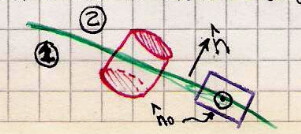
\includegraphics[width=0.4\textwidth]{images/fig_ft1_contornos_medios.jpg}

Aplicando teorema de Stokes sobre el rotor de $\vb{H}$ para el circuitito
diminuto se tiene
\[
	\int_S \rotorm{H}\cdot \hat{n} \: dS = (\vb{H}_2 - \vb{H}_1) \cdot d\Bell
\]
pero como 
\[
	\frac {d\Bell} {d\ell} = d\hat{\ell} = \hat{n}_0 \times \hat{n}
\]
y será (tendiendo a cero la superficie del circuitito)
\[
	(\vb{H}_2 - \vb{H}_1) \cdot ( \hat{n}_0 \times \hat{n} ) d\ell =
	d\ell \hat{n}_0 \cdot [ \: \hat{n} \times (\vb{H}_2 - \vb{H}_1) \: ]
\]
Como la orientación de $\hat{n}_0$ es arbitraria los dos miembros son iguales y
entonces
\[
	\hat{n} \times (\vb{H}_2 - \vb{H}_1) = \frac{4\pi}{c} \vb{g}_L 
\]
que nos dice que el componente tangencial de \vb{H} no es continuo cuando circula
por el borde una $\vb{g}_L$.


Si esta es nula se tiene
\[
	\begin{cases}
	B_{n2} = B_{n1} \\
	\\
	\displaystyle B_{t2} = \frac{\mu_2}{\mu_1}\: B_{t1}
	\end{cases}
	\qquad 
	\begin{cases}
	\displaystyle H_{n2} = \frac{\mu_2}{\mu_1}\: H_{n1} \\
	\\
	H_{t2} = H_{t1} 
	\end{cases}
\]

\subsection{Imán permanente}

Hay magnetización \vb{M} aún en ausencia de campo. No es un medio lineal de modo que
\[
	\vb{M}	 \neq \xi_M \vb{H} \Rightarrow \vb{B} \neq \mu \vb{H}
\]
El campo \vb{M} es fuente de campo. El asunto es que $\vb{M}$ tiene el problema de
la discontinuidad, pero $ \vb{M} = 0 $ fuera del medio.
La relación entre \vb{B},\vb{H} depende de la historia del medio.
\[
	\frac{1}{c}\vb{J}_M = \rotorm{M}
\]
si \vb{J}$_L=0$ entonces 
\[
	\rotorm{H} = 0 \qquad \Rightarrow \vb{H} = -\Nabla\phi_m
\]
que es un potencial escalar magnético.
\[
	\Nabla\cdot( \vb{H} + 4\pi\vb{M} ) = \divem{B} = 0
\]
\[
	\divem{H} = -4\pi\divem{M}
\]
\[
	-\nabla^2 \phi_m = -4\pi\divem{M}
\]
\[
	\nabla^2 \phi_m = -4\pi\rho_m
\]
donde se ha definido cargas ficticias de magnetización.
Se deduce una $ \sigma = \vb{M} \cdot \hat{n} $.

\[
	\divem{M} \equiv -\rho_m \qquad \qquad \vb{M}\cdot\hat{n} \equiv \sigma_m
\]
\[
	\phi_m = \frac{1}{c} \int_{S'} \frac{\vb{M}}{|\vb{x}-\vb{x}'|} \cdot d\vb{S}' -
		\frac{1}{c} \int_{V'} \frac{\divem{M}}{|\vb{x}-\vb{x}'|} dV' 
\]
\[
	\vb{A}( \vb{x}) = \frac{1}{c} \int_S \frac{ \vb{M}\times\hat{n} }{|\vb{x}-\vb{x}'|} d\vb{S}' - 
		\frac{1}{c} \int_V \frac{ c(\rotorm{M}) }{|\vb{x}-\vb{x}'|}  dV'
\]
Estas dos soluciones son equivalentes.
\[
	\phi_m = \frac{1}{c} \int_{V'} \frac{\rho_L}{|\vb{x}-\vb{x}'|}  dV' +
		\frac{1}{c} \int_{V'} \frac{ \vb{P}\cdot(\vb{x}-\vb{x}')}{|\vb{x}-\vb{x}'|^3} dV' 
\]
pero el integrando del segundo término se puede reescribir como 
\[
	-\vb{P}\cdot\Nabla\left(\frac{1}{|\vb{x}-\vb{x}'|}\right)
\]
de manera que 
\[
	\phi_m = \frac{1}{c} \int_{V'} \frac{\rho_L}{|\vb{x}-\vb{x}'|}  dV' -
		\frac{1}{c} \int_{V'} \frac{ \divem{P}) }{|\vb{x}-\vb{x}'|} dV' 
\]
\[
	\phi_m = \frac{1}{c} \int_{V'} \frac{1}{|\vb{x}-\vb{x}'|}( \rho - \divem{P} )  dV'
\]
se puede asociar
\[
	\divem{P} = \rho_P.
\]

% Sueltos:
% \[
% 	\vb{A}( \vb{x}) = \frac{1}{c} \int_V \left[ \frac{ \vb{J}_L(\vb{x}') }{|\vb{x}-\vb{x}'|} +
% 		\frac{ c \vb{M} \times (\vb{x}-\vb{x}') }{|\vb{x}-\vb{x}'|^3} \right] dV'
% \]
% \[
% 	\vb{A}( \vb{x}) = \frac{1}{c} \int_V \left[ \frac{ \vb{J}_L(\vb{x}') }{|\vb{x}-\vb{x}'|} +
% 		\frac{ c \divem{M} }{|\vb{x}-\vb{x}'|} \right] dV'
% \]
% \[
% 	\vb{A}( \vb{x}) = \frac{1}{c} \int_V \frac{ \vb{J}_L(\vb{x}') + \vb{J}_M(\vb{x}' ) }{|\vb{x}-\vb{x}'|}	
% \]

\begin{figure}[htb]
	\begin{center}
	\includegraphics[width=0.6\textwidth]{images/fig_ft1_magnetizaciones.pdf}	 
	\end{center}
	\caption{}
\end{figure}


% =================================================================================================
\section{Polarización y magnetización de medios}
% =================================================================================================

La polarización y la magnetización suelen depender de los campos externos, es decir 
$\vb{P}=\vb{P}(\vb{E})$ y $\vb{M}=\vb{M}(\vb{H})$.
Una sustancia lineal admite un desarrollo del tipo
\[
	\vb{M} \approx M_{0i} + \left.\dpar{M_i}{H_j}\right|_{H=0} H_j
\]
\[
	\vb{P} \approx P_{0i} + \left.\dpar{P_i}{E_j}\right|_{E=0} E_j
\]
y como en general vale que $\vb{M}_0=0, \vb{P}_0=0$  se da que 
\[
	\vb{M} = \sum_i \sum_j \left( \left.\dpar{M_i}{H_j}\right|_{H=0} H_j \right) 
\]
\[
	\vb{M} = 
	\begin{pmatrix}
	 \displaystyle{\dpar{M_x}{H_x}} & \displaystyle{\dpar{M_x}{H_y}} & \displaystyle{\dpar{M_x}{H_z}} \\
	 \displaystyle{\dpar{M_y}{H_x}} & \displaystyle{\dpar{M_y}{H_y}} & \displaystyle{\dpar{M_y}{H_z}} \\
	 \displaystyle{\dpar{M_z}{H_x}} & \displaystyle{\dpar{M_z}{H_y}} & \displaystyle{\dpar{M_z}{H_z}}
	\end{pmatrix}
	\begin{pmatrix}
	 \displaystyle{H_x} \\
	 \\
	 H_y \\
	 \\
	 H_z
	\end{pmatrix}
\]
y ahí se ve explícitamente que tienen que ser tensores,
\[
	\vb{M} = \overleftrightarrow{\xi}_M \vb{H} \qquad\qquad 
	\vb{P} =  \overleftrightarrow{\xi}_e \vb{E}.
\]

Estos tensores son, respectivamente, los tensores de susceptibilidad magnética y
eléctrica. En el caso en que sean escalares (isotropía [¿?]) la susceptibilidad
eléctrica solo puede tomar valores positivos mientras que la magnética puede
tomar también valores negativos.

\subsubsection{Medios magnéticos de muy alta permeabilidad}

Consideremos un caso especial donde
\[
	\vb{g}_L = 0.
\]
Entonces
\[
	\hat{n}\times\vb{H}_1 = \hat{n}\times\vb{H}_2
\]
\[
	\vb{B}_1\cdot\hat{n} = \vb{B}_2\cdot\hat{n} \qquad
		\mu_1\vb{H}_1\cdot\hat{n} = \mu_2\vb{H}_2\cdot\hat{n}
\]
\[
	H_{2n} = \frac{\mu_1}{\mu_2} H_{1n} \quad \text{si} \; \mu_1 \gg \mu_2 \Rightarrow H_2 \gg H_1
\]
En el límite $\vb{H}_2 \perp$ superficie del medio y es similar al \vb{E} a la salida de un
conductor; las superficies de materiales de permeabilidad muy alta son aproximadamente {\it equipotenciales}.

\begin{figure}[htb]
	\begin{center}
	\includegraphics[width=0.9\textwidth]{images/fig_ft1_medios1.pdf}	 
	\end{center}
	\caption{}
\end{figure}

Para medio anisótropo
\[
	D_i = \epsilon_{ij} E_j \qquad \text{es decir} \quad \vb{D} = \overleftrightarrow{\epsilon} \vb{E}
\]
\notamargen{Esto estaba en las inmediaciones
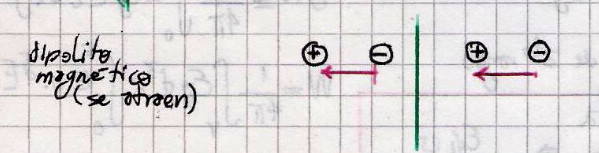
\includegraphics[width=0.35\textwidth]{images/fig_ft1_picdipolitos.jpg}
}

\subsubsection{Consideraciones en medios magnéticos}

Fuera de un imán permanente 
\[
	\rotorm{B} = 0 = \frac{4\pi}{c}\vb{J}_T
\]
y entonces parecería que podemos definir un
\[
	\vb{B} = -\Nabla \phi_m^B,
\]
pero fallará en la superficie de separación donde hay \vb{J}$_m$ y por ende \vb{J}$_T$. Lo que sí funciona
es
\[
	\rotorm{H} = 0 = \frac{4\pi}{c}\vb{J}_L
\]
que vale dentro y fuera del imán.
\begin{figure}[htb]
	\begin{center}
	\includegraphics[width=0.25\textwidth]{images/fig_ft1_medios2.pdf}	 
	\end{center}
	\caption{}
\end{figure}

Entonces
\[
	\vb{H} = -\Nabla \phi_m^H,
\]
y
\[
	\divem{H} = -\Nabla(\Nabla \phi^H_m ) = -4\pi \divem{M} = 4\pi\rho_M
\]
\[
	-\nabla^2 \phi_m^H = 4\pi\rho_M
\]
una ecuación de Poisson para el potencial $\phi_m^H$.

\[
	(\vb{B}_2 - \vb{B}_1)\cdot\hat{n} = 0
\]
\[
	(-\Nabla \phi^2_H + \Nabla \phi^1_H - 4\pi \vb{M})\cdot\hat{n} = 0
\]
\[
	(-\Nabla \phi^2_H + \Nabla \phi^1_H )\cdot\hat{n} = 4\pi \vb{M}\cdot\hat{n} = 4\pi \sigma_M
\]

\begin{ejemplo}{\bf Problema 5 (imán esférico)}

Calculamos todo de varias maneras

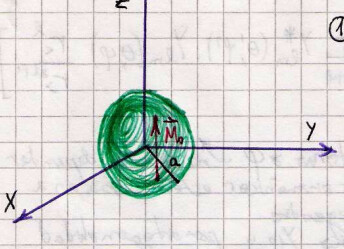
\includegraphics[width=0.25\textwidth]{images/fig_ft1_imanesferico_A.jpg}

Bola \textcircled{1}
\[
	\vb{m} = \int \vb{M} \: dV = \frac{4 \pi a^3 }{3} M_0 \hat{z}
\]

Bola \textcircled{2}
\[
	\rotorm{H} = 0 \qquad \qquad \divem{H} = 4 \pi \rho_m
\]
\[
	\vb{m} = \int \rho_m \vbx dV = \hat{z} \int \rho_m \: z \: dV
\]
Se tienen además
\[
	\rho_m = - \divem{M} \qquad \sigma_M = \vb{M}\cdot{\hat{n}}
\]
y como \vb{M} es constante en el interior, no hay $\rho_m$ en el volumen.
Habría que escribir bien la magnetización \vb{M}.
Usaremos una función escalón

Consideramos una función escalón $ \Theta $ de tal manera que 
\[
	\vb{M} = M_0 \hat{z} \Theta(a-r)
\]
donde 
\[
	M_0 \hat{z} = M_0 ( \cos\theta \hat{r} - \sin\theta \hat{\theta} ) \Theta(a-r)
\]
según puede verse en el figurín bajo estas líneas (se ve solo el tetón).

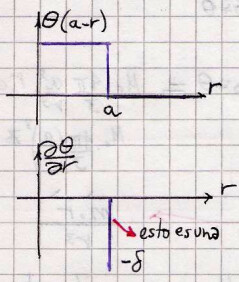
\includegraphics[width=0.25\textwidth]{images/fig_ft1_imanesferico_B.jpg}

Entonces,
\[
	\divem{M} = M_0 \left( 
	 \frac{1}{r^2}\dpar{}{r}[ r^2 \cos\theta \Theta(a-r) ] -
	 \frac{1}{r\sin\theta}\dpar{}{\theta}[ \sin^2\theta \Theta(a-r) ]
	\right) = - M_0 \cos\theta \delta(r-a)
\]
donde $ M_0 \cos\theta = \sigma_M $ resultado que es consistente con la cuenta de
$\sigma = \vb{M}\cdot\hat{n}$.

Finalmente,
\[
	\vb{m} = \int \rho_m z dV = M_0 \int_0^{2\pi} \int_0^\pi \: a^3\cos^2\theta \sin\theta d\theta d\vp
	= 2 \pi M_0 a^3 \int_{-1}^1 x^2 dx = \frac{4\pi}{3} M_0 a^3 \zver
\]

Bola \textcircled{3}. Se ilustra en la postal siguiente

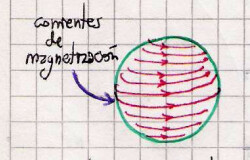
\includegraphics[width=0.25\textwidth]{images/fig_ft1_imanesferico_C.jpg}
Desde
\[
	\vb{J}_m = c \rotorm{M}
\]
se deduce
\[
	\vb{g}_m = c \vb{M}\times \hat{n} = c M_0 \zver\times\rver = cM_0\sin\theta \phiver
\]
\[
	\vb{m} = \frac{1}{2c}\int \pv{x}{J}_m \: dV = \frac{I}{2c} \int \vbx \times d\Bell =  
	\frac{I \text{ Area }}{c}\zver
\]
y hemos obtenido el resultado de \vb{m} como área por corriente.

Para el anillete mostrado en el cartón

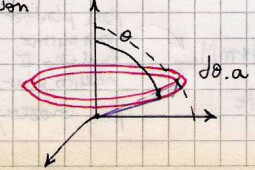
\includegraphics[width=0.25\textwidth]{images/fig_ft1_imanesferico_D.jpg}

\[
	d\vb{m} = \frac{\text{seccion}}{c} du =
	\frac{1}{c} \pi a^2 \sin^2\theta \: a \: \vb{g}_m d\theta
\]
o bien, integrando,
\[
	\vb{m} = \zver \int_0^\pi \: M_0 \pi a^3 \sin^3\theta \: d\theta = 
	\zver \left( \frac{4 \pi }{3} a^3 M_0 \right)
\]
con lo cual el potencial resulta
\[
	\phi_M = \int \: \frac{ \rho_m }{ | \vbx - \vbx' | } \: dV
\]
o en full splendor
\[
	\phi_M = \int \int M_0 \: \cos\theta
	\left[ \sum_{\ell=0}^\infty \sum_{m=-\ell}^\ell \frac{4\pi}{2\ell+1} 
	Y_{\ell m}^*(\theta',\vp') Y_{\ell m}(\theta,\vp) 
	\frac{r_<^\ell}{r_>^{\ell+1}} \right]
	a^2 \sin\theta \: d\theta d\vp.
\]

Aquí hay simetría en torno a \vp de manera que el problema no puede depender de esta
coordenada. Los armónicos esféricos pasan a ser los polinomios de Legendre. Puedo ver
que $\cos\theta$ es un armónico $Y_{10}$ y por ortogonalidad se va toda la doble
sumatoria y sobreviven solamente $\ell=1, m=0$.

\notamargen{Valen $\cos\theta = Y_{10} \sqrt{ 4 \pi / 3 }$.}
Usando esta información tenemos
\[
	\phi_M = M_0 a^2 \Frac{r_<}{r_>^2} \sqrt{ \frac{ 4\pi }{ 3 } } \frac{4\pi}{3} 
	Y_{10}^*(\theta,\vp) =
	M_0 \frac{4\pi}{3} a^2 \frac{r_<}{r_>^2} \cos\theta
\]
solución que es válida en todo el espacio.
\[
	\phi_{M} = \begin{cases}
		\displaystyle M_0 \frac{ 4 \pi a^2 }{3} \frac{r}{a^2} \cos\theta \qquad r < a \\
		\\
		\displaystyle M_0 \frac{ 4 \pi a^2 }{3} \frac{a}{r^2} \cos\theta \qquad r > a
	\end{cases}
\]
donde el último caso $r>a$ se puede escribir como
\[
	M_0 \frac{ 4 \pi }{3} \Frac{a}{r}^3 z = \frac{\pe{m}{r}}{|x|^3}
\]

Recordemos que si $ r>a $ es $\vb{B}=\vb{H}$ mientras que para $r<a$ es $\vb{B} = \vb{H} + 4\pi \vb{M}$.

Si introducimos este imán pelota en un medio tengo una alteración en el contorno.
Aquí hay que usar separación de variables.
\[
	\phi_I = \sum_\ell \: A^I_\ell \: r^\ell \: P_\ell(\cos\theta)
\]
\[
	\phi_{II} = \sum_\ell \: \frac{B^{II}_\ell}{r^{\ell+1}} \: P_\ell(\cos\theta)
\]
donde en $I$ se ha tirado una parte de la solución porque diverge en cero, mientras que en $II$ se tira
en cambio la parte que corresponde.

Los contornos salen de evaluar
\[
	\phi_I(a,\theta) = \phi_{II}(a,\theta)
\]
lo cual conduce a 
\[
	A^I_\ell = \frac{B_\ell^{I}}{a^{2\ell+1}}
\]

En el caso de los campos $\vb{B}$ se tendrá $B_{nII} = B_{nI}$ que conduce a [¿?]
\[
	\mu H_{nI} = H_{nII} + 4 \pi M_{nI}
\]
donde el lhs no se puede plantear en un imán permanente y el rhs implica que para plantear
esto mismo en el caso $II$ necesito conocer $M$ pero conozco $\mu$.
\[
	- \mu \dpar{\phi_{II}}{r} + \dpar{\phi_{II}}{r} = 4 \pi M_0 \cos\theta = 4 \pi \sigma_M
\]
donde esta última ecuación es casi una de contorno como para el campo \vb{E}  pero ojo que
está el $\mu$. Viene de que $\vb{H} = - \nabla\phi$.
Luego,
\[
	\sum_{\ell=0}^\infty \: 
	\left[ \mu(\ell+1) \frac{B^{II}_\ell}{a^{\ell+2}} + \ell a^{\ell-1} A_\ell^I \right] 
	P_\ell (\cos\theta) =  4 \pi \sigma_M
\]
y ahora se aplica ortogonalidad multiplicando por $P_{\ell'}$ e integrando, entonces
\[
	c_\ell \frac{2}{2\ell +1} \delta_{\ell\ell'} = \frac{4\pi M_0}{2\ell'+1} \delta_{\ell 1}
	\qquad \qquad  2 \mu \frac{B_1}{a^3} + A_1 = 4 \pi M_0
\]
y de estas dos ecuaciones se obtienen los coeficientes
\[
	A^I_\ell = \frac{B_\ell^{I}}{a^{2\ell+1}}
\]
sumados a
\[
	4\pi M_0 = (1+2\mu) A \qquad A_1 = \frac{4 \pi M_0}{1+2\mu} \qquad B_1 = \frac{4 \pi M_0 a^3}{1+2\mu}
\]

Finalmente,
\[
	\phi = \begin{cases}
		\displaystyle \frac{4 \pi M_0}{1+2\mu}\: r \:\cos\theta \quad \qquad r < a \\
			\\
		\displaystyle \frac{4 \pi M_0}{1+2\mu}\: \frac{a^3}{r^2} \:\cos\theta \quad \qquad r > a
		\end{cases}
\]
donde otra vez la última expresión, para $ r > a $, tiene la forma $ \pe{m}{x}/|x|^3$ donde
$\vb{m} = 4 \pi M_0 a^3 \zver /(1+2\mu)$.

Un momento dipolar magnético diferente al inicial es porque hubo momento inducido
\[
	\vb{m}_{\text{ind}} = \vb{m}_T - \vb{m} =
	\left( \frac{4 \pi a^3}{1+2\mu} M_0 - \frac{4 \pi a^3}{3} M_0 \right) \zver
\]
\[
	\vb{m}_{\text{ind}} = \Frac{1-\mu}{1 + 2\mu} \frac{8\pi}{3} a^3 M_0 \zver
\]
 
\end{ejemplo}

\subsection{Desarrollo dipolar del campo magnético}

El potencial vector de un dipolo es
\[
	\vb{A}(\vb{x}) = \frac{\vb{m}\times(\vb{x}-\vb{x}')}{|\vb{x}-\vb{x}'|^3} = \vb{m} \times \Nabla 
		\frac{1}{|\vb{x}-\vb{x}'|}
\]
Supongo que integrando esto en volumen y usando partes se arriba a
\[
	\vb{A}(\vb{x}) = \int_{V'} \frac{\rotorm{\vb{M}}}{|\vb{x}-\vb{x}'|} dV' -
	\int_{V'} \Nabla \times \frac{\vb{M}}{|\vb{x}-\vb{x}'|} \: dV'
\]
Entonces, usando la identidad {\bf ID 3} del apéndice se convierte en
\[
	\vb{A}(\vb{x}) = \int_{V'} \frac{\rotorm{\vb{M}}}{|\vb{x}-\vb{x}'|} dV' +
			\int_{S'} \frac{\vb{M}\times\hat{n}}{|\vb{x}-\vb{x}'|} dS'
\]
y se pueden pensar que el término de volumen se debe a una corriente de magnetización 
$\vb{J}_M$ y el de superficie a una corriente superficial $\vb{g}_M$, de modo que
se tiene
\[
	\vb{A}(\vb{x}) = \frac{1}{c} \int_{V'} \frac{\vb{J}_M}{|\vb{x}-\vb{x}'|} dV' +
			\frac{1}{c} \int_{S'} \frac{\vb{g}_M}{|\vb{x}-\vb{x}'|} dS'
\]
El término de superficie puede ser fácil si se conoce $\vb{M}$ sobre la superficie.
Este componente se puede dejar de lado si se toma una región de integración que
engloba a toda la distribución.
\notamargen{Esto puede ser el kid de lo que no entendía y de esos dibujillos en
la carpeta
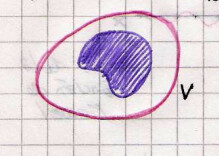
\includegraphics[width=0.2\textwidth]{images/fig_ft1_regionintegracion.jpg}
}

Las unidades de $\vb{g}_M$ tienen que ser de corriente sobre longitud ($q/(t\ell)$ 
o bien $i/\ell$).

Me falta descular esta expresión, pero tendría que ser la expresión anterior luego
de cosmética y tirar el término de superficie. Veremos
\[
	\vb{A}(\vb{x}) = \int_{V'} \vb{\mathcal{M}}(\vb{x}') \times \Nabla 
			\left(\frac{1}{|\vb{x}-\vb{x}'|}\right) dV'
\]
Es el potencial vector de una distribución de momento dipolar magnético con densidad
$ \vb{M}(\vb{x}')$

% =================================================================================================
\subsection{Campo externo sobre distribución}
% =================================================================================================

Se quiere ver la maquinaria matemática para evaluar el efecto de un campo externo sobre
una configuración de carga.
Recuérdese que un campo homogéneo no hace fuerza sobre un dipolo.
El punto de partida es la integral del potencial
\[
	W = \int \rho(\vbx) \phi(\vbx) d^3x
\]
y el potencial
\[
	\phi(\vbx) = \phi(0) + \vbx \cdot \Nabla\phi(0) + 
	\frac{1}{2} x_i x_j \partial_i \partial_j \phi(0) + ...
\]
\[
	\phi(\vbx) = \phi(0) + \vbx \cdot \vb{E}(0) + 
	\frac{1}{2} x_i x_j \partial_i \vb{E}_j(0) + ...
\]

Implantando esta expansión en la integral previa,
\[
	W = \phi(0) \int \rho(\vbx) d^3x - \vb{E}(0) \int \vbx \rho(\vbx) d^3x 
	- \frac{1}{6} Q_{ij}  \partial_i \vb{E}_j(0)
\]
\[
	W = q \phi - \pe{p}{E} - \frac{1}{6} Q_{ij} \partial_i \vb{E}_j 
\]
Tomando el gradiente, con su signo, $ \vb{F} = - \Nabla W $ y
entonces
\[
	F_k = - \partial_k W =
	-q \:\partial_k \phi + p_i \partial_k E_i + \frac{1}{6} Q_{}ij\partial_i\partial)j E_k
\]
entonces $ \partial_k E_j = \partial_j E_k $ puesto que el carácter irrotacional del
campo externo hace que puedan intercambiarse los índices en la expresión.
El primer término del rhs es $q\vb{E}$.


% =================================================================================================
\section{Consideraciones energéticas}
% =================================================================================================

Aquí la idea es construir la configuración carga a carga. Evaluando el trabajo de
generar el potencial total.
Recordemos [¿?]
\[
	\vb{F} = q \vb{E} = q (-\Nabla\phi) = - \Nabla U
\]
\[
	\Delta U = W = \int_\Gamma \vb{F}\cdot d\vb{\ell} \rightarrow \Delta U = 
	- \int_\Gamma \Nabla (q\phi) \cdot d\vb{\ell} = -q \Delta \phi
\]
\[
	\delta U = \vb{F}\cdot\delta\vb{x} \qquad\qquad  \frac{\delta U}{\delta x} = F_t
\]
donde el subíndice es por tangencial.

Se empieza con $W_1 = 0 $. Luego
\[
	W_2 = q_2 \frac{q_1}{r_{12}} = \frac{1}{2}( W_2^a + W_2^b ) =
	\frac{1}{2}\left( q_1 \frac{q_2}{r_{12}} + q_2 \frac{q_1}{r_{21}} \right)
\]
\[
	W_3 = q_2 \frac{q_1}{r_{12}} + q_3 \frac{q_1}{r_{13}} + q_2 \frac{q_3}{r_{23}}
\]
\[
	W_3 = \frac{1}{2}\left( q_1 \frac{q_2}{r_{12}} + q_1 \frac{q_3}{r_{13}} + q_2 \frac{q_1}{r_{21}}
		+ q_2 \frac{q_3}{r_{23}} + q_3 \frac{q_1}{r_{31}} + q_3 \frac{q_2}{r_{32}} \right)
\]
\[
	W_N = \sum_{i\neq j}^N \frac{1}{2}\frac{q_i q_j}{r_{ij}} =
	\sum_{i,j}^N \frac{1}{2} q_i \phi_{ij}[ 1 - \delta_{ij}]
\]
siendo $\phi_{ij}$ el potencial sobre $q_i$ debido a $q_j$.
Entonces,
\[
	W_N = \frac{1}{2} \sum_i^N  q_i \phi_i 
\]
es el potencial de todas las cargas producido en la posición de $q_i$.
La versión continua será, evidentemente,
\[
	W = \frac{1}{2} \int_V \rho(\vb{x}) \phi(\vb{x}) dV
\]
Supongamos ahora la presencia de un medio material.
Se quiere ver que trabajo $W$ debe hacerse para modificarlo en un $\Delta \rho$.
\[
	\delta W = \frac{1}{2} \: \rho \: \delta V \phi,
\]
o bien
\[
	\Delta(\delta W) = \delta q \: \phi =  \delta \rho \: dV \: \phi.
\]
Se integra en todo el volumen,
\[
	\delta W = \int \: \delta \rho\: \phi \: dV.
\]
que satisface $\divem{D}=4\pi\rho_L$ de modo que
\[
	\delta W = \frac{1}{2}\frac{\Nabla\cdot(\delta\vb{D})}{4\pi} \delta V \phi 
\]
o bien
\[
	\delta W = \frac{1}{4\pi} \int \: \Nabla \cdot \delta \vb{D} \: \phi \: dV.
\]
y usando identidades (la de siempre -ponerla en Apéndice- o partes)
\[
	\delta W = \frac{1}{4\pi} \left( 
	\int \: \Nabla \cdot ( \delta \vb{D} \: \phi ) \: dV -
	\int \: \delta\vb{D} \cdot \Nabla \phi \: dV
	\right)
\]
Ahora se presupone que se integra en todo el espacio. La superficie en el infinito
tiene $\phi,\vb{D}$ tendiendo a cero y me olvido de esa integral. Entonces, reemplazando
el gradiente del potencial por el campo, se tiene
\[
	\delta W =  \frac{1}{4\pi}  \int \: \delta\vb{D} \cdot \vb{E} \: dV =
	\frac{1}{4\pi}  \int \: \left( \int_0^D \vb{E} \cdot \delta\vb{D} \right) \: dV
\]
y esto es el trabajo necesario para formar la configuración en presencia de medios
materiales.
Resquechos de la otra deducción [habría que consolidar] siguen a continuación:
\[
	\Nabla\cdot(\delta\vb{D}\phi) = \delta\vb{D} \cdot \Nabla\phi  + \phi \Nabla\cdot\delta\vb{D}
\]
\[
	\delta W = \frac{1}{8\pi} \delta V [\Nabla\cdot(\delta\vb{D}\phi) - \delta\vb{D} \cdot \Nabla\phi ]
\]
\[
	W = \frac{1}{8\pi}\left( \int_V \Nabla\cdot(\vb{D}\phi)dV + \int_V \vb{D}\cdot\vb{E} dV \right)
\]
pero la primera integral se pasa a una de superficie según
\[
	\int_S \vb{D}\phi dS
\]
y si la misma es muy grande tiende a cero. Entonces quedamos en que 
\[
	W = \frac{1}{8\pi} \int_V \vb{D}\cdot\vb{E} dV
\]
que es el trabajo necesario para formar una configuración en presencia de medios materiales. Vale
para medios lineales, sin imponer isotroía u homogeneidad.

Este cálculo es a temperatura constante, el medio material no altera su $\epsilon$.
Es un proceso isotérmico. Uno asume que $\epsilon=\epsilon(\vb{x})$ y no varía con el tiempo.
En la práctica $\epsilon$ varía con la temperatura.

\subsection{Medios anisótropos}

Consideremos un medio lineal anisótropo
\[
	D_i = \varepsilon_{ij} E_j
\]
con el tensor de segundo rango $\varepsilon_{ij}$. En este caso
\[
	\delta W = \frac{1}{4\pi} \int  \varepsilon_{ij} E_i \delta E_j \qquad \qquad
	W =  \frac{1}{4\pi} \int \varepsilon_{ij} dV \int_0^E E_i \delta E_j
\]
en la cual el campo \vb{E} desde cero a su valor final es paralelo a si mismo en todo
momento.

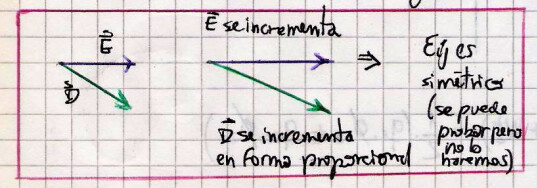
\includegraphics[width=0.25\textwidth]{images/fig_ft1_mediolinealanisotropo.jpg}

Entonces
\[
	\frac{\delta E_i}{\cos\alpha_i} = \frac{\delta E_j}{\cos\alpha_j}
\]
\[
	\delta E_j = a_{ij} \delta E_i 
\]
con $a_{ij} = \cos\alpha_j / \cos\alpha_i$. Entonces $E_j = a_{ij} E_i = a^{ij} E_i$ y 
\notamargen{¿Qué será el $a$ contravariante?}
\[
	 \int_0^E E_i \delta E_j =  a^{ij} \int_0^E E_i \delta E_i = \frac{1}{2}  a^{ij} E_i^2
\]
de modo que también
\[
	\int_0^E E_i \delta E_j = \frac{1}{2} E_i E_j,
\]
y entonces
\[
	W = \frac{1}{4\pi} \int \frac{1}{2} \varepsilon_{ij} E_i E_j  dV =
	\frac{1}{8\pi} \int \pe{E}{D} \: dV.
\]

Esta expresión vale para medios lineales isótropos o no homogéneos o no homogéneos.
Es decir, es bastante general.
Traemos cargas desde el infinito pensando que el medio material no cambia su constante
(temperatura constante), por ello indirectamente hemos supuesto un proceso isotérmico.
Este trabajo ha incrementado la función libre de Helmholtz.

% =================================================================================================
\section{Interpretación termodinámica de U}
% =================================================================================================

El incremento de energía a T constante
\be
	\delta W = U = \frac{1}{8 \pi} \vb{E}\cdot\vb{D} = \frac{1}{8 \pi} \epsilon_{ij}E_i E_j	\qquad
	\text{con} \; \epsilon_{ij} = \epsilon_{ji} \; \text{tensor simétrico}
	\label{energíaEM}
\ee
Pero $\epsilon$ es función de T la temperatura y entonces no podemos decir que
\[
	dU = dW
\]
valga en general, pues también hay variación del calor (a no ser que sea un proceso isotérmico) de modo que 
la energía que representa \eqref{energíaEM} es la energía libre de Helmholtz a T constante.
\[
	dU = dQ - dW \qquad \qquad F = U - TS
\]
\[
	dF = dU - TdS - SdT
\]
pero al ser la última cero, resulta
\[
	dF|_T = dU - T.dS = \frac{1}{8\pi} \int_V \vb{E}\cdot\delta\vb{D} dV
\]
\[
	dF = \frac{1}{8\pi} \int_V \vb{E}\cdot\delta\vb{D} dV - SdT
\]
de modo que como el primer término es $\partial F / \partial D |_T$ resulta que 
la entropía es
\[
	S = -\left.\dpar{F}{T}\right|_D
\]

Si es un medio isótropo entonces $\vb{D} = \epsilon \vb{E}$ y, se puede escribir 
\[
	F = \frac{1}{8\pi} \int_V \frac{1}{\epsilon}\vb{D}\cdot\vb{D} dV
\]
entonces
\[
	S = \left.\dpar{F}{T}\right|_D	= \frac{1}{8\pi} \int_V \vb{D}\cdot\vb{D} 
		\dpar{}{T} \left( \frac{1}{\epsilon} \right) dV
\]
\[
	=  - \frac{1}{8\pi} \int_V \vb{D}\cdot\vb{D} \frac{1}{\epsilon^2} \dpar{\epsilon}{T}  dV =
	-\frac{1}{8\pi} \int_V \vb{E}\cdot\vb{D} \frac{1}{\epsilon} \dpar{\epsilon}{T} \: dV. 
\]
\notamargen{Estamos queriendo ver el calor absorbido por el sistema si el campo E crece a su valor final.}
De esta manera  
\[
	U = F + TS = \frac{1}{8\pi} \int_V \vb{D}\cdot\vb{D} \frac{1}{\epsilon} dV  +
	\frac{1}{8\pi} \int_V \vb{E}\cdot\vb{D} \frac{1}{\epsilon} \dpar{\epsilon}{T}  dV 
\]
\[
	U = \frac{1}{8\pi} \int_V \frac{1}{\epsilon} \left[ \vb{D}\cdot \left( \vb{D} + 
		\vb{E} \dpar{\epsilon}{T} T \right) \right] dV  = \frac{1}{8\pi} \int_V \frac{1}{\epsilon}
		\vb{D}\cdot \vb{E} \left[ \epsilon + T \dpar{\epsilon}{T}  \right] dV,
\]
\notamargen{Agitación térmica tiende a desorientar dipolos.}
y finalmente para medios lineales e isótropos
\[
	U = \frac{1}{8\pi} \int_V \frac{1}{\epsilon} \vb{D}\cdot \vb{E} \dpar{ (T \epsilon) }{T} dV
\]
y la segunda ley de la termodinámica es
\[
	\delta Q = T.dS = \frac{1}{4\pi} \int_V \vb{E}\cdot\delta\vb{D} \frac{T}{\epsilon}
	\dpar{\epsilon}{T} dV
\]
con $\epsilon > 0, T > 0,$ (lo cual vale siempre) $ \partial \epsilon / \partial T < 0$ si el $\epsilon$ 
decrece con T el cuerpo se enfría $\delta Q < 0$.
\notamargen{Isotropía implicará noigual dirección de \vb{D,E} pero no pueden ser opuestos [¿?].}

Este análisis está en el libro de Panofsky y en el Landau de electrodinámica de los medios.

\subsection{Fuerza entre placas de un condensador}

Sea un medio inmerso en un sistema aislado del exterior. Entonces tendremos $dW_e + dW_m =0$ de lo
cual deducimos
\[
	dW_m = \vb{F}\cdot d\vbx = -dW_e,
\]
o bien
\[
	\vb{F} = - \nabla W_e|_q
\]
que pasa para un sistema aislado a carga constante.
Para un condensador
\[
	W_e = \frac{1}{2c} Q^2 \qquad \qquad -\Nabla W_e = \frac{1}{2} \frac{Q^2}{C^2} \Nabla C = \vb{F}
\]
que es la energía electrostática proveniente de Helmholtz.
\[
	\vb{F}\cdot d\vbx + \delta W_e|_V + dW_B = 0
\]
donde el segundo y tercer término son a tensión constante y el trabajo de la batería, respectivamente.
Entonces
\[
	\vb{F} = \nabla W_e|_V,
\]
que es un proceso a $V$ constante; la fuerza tiende a aumentar la energía libre de Helmholtz del
sistema, aunque la fuerza entre placas continúa siendo la misma.
La ilustración ilustra

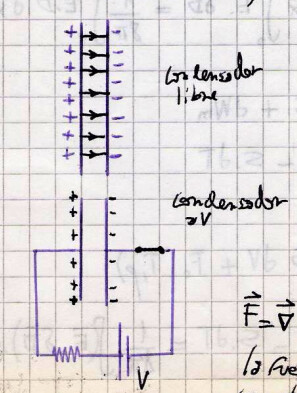
\includegraphics[width=0.25\textwidth]{images/fig_ft1_fuerza_placas_condensador.jpg}

La fuerza tiende a deformar el condensador, pero aumenta la capacidad.
Luego,
\[
	W_e = \frac{1}{2} C V^2
\]
\[
	\vb{F} = \nabla W_e|_V = \frac{1}{2} V^2 \Nabla C = \frac{1}{2} \frac{Q^2}{C^2} \Nabla C
\]


% =================================================================================================
\section{Teorema de Thomson}
% =================================================================================================

Consideremos una zona del espacio donde hay un campo eléctrico con un conductor.
Al llegar al equilibrio se redistribuyen las cargas para hacer mínimo la energía libre de
Helmholtz $F$ del sistema.

La variación de la energía para un sistema de $ n $ electrodos será
\[
	\delta W = \int_V \: \phi \: \delta\rho \: dV  =
	\sum_{i=1}^n \: \int \: \phi_i \: \delta\rho_i \: dV =
	\sum_{i=1}^n \: \phi_i \: \int \:  \delta\rho_i \: dV = 0
\]
donde $\delta\rho$ es la variación de la densidad de carga y donde se ha sumado en los 
equipotenciales $\phi_i$ para cada conductor $i$-ésimo. La última igualdad se hace 
cero porque los conductores están aislados y su carga neta no varía su distribución.

\[
	\delta W = \frac{1}{8\pi} \int_V \vb{E}\cdot\delta\vb{D} dV = \frac{1}{8\pi} \int_V \left( 
-\Nabla\phi\cdot\delta\vb{D}  dV \right)  = 
\]
\[
	\delta W = \frac{1}{8\pi} \int_V \left[ \phi \Nabla\cdot\delta\vb{D} - 
			\Nabla\cdot\delta(\vb{D}\phi) \right] dV
\]
\[
	\delta W = \frac{1}{8\pi} \sum_i^N \int_V \phi_i 4\pi \delta p_i dV - 
		\frac{1}{8\pi} \int_{\partial V} \vb{D}\phi \cdot d\vb{S} =
		\frac{1}{2} \sum_i^N  \phi_i \int_V \delta \rho_i dV = 0
\]
y la integral de superficie la podemos dejar desvanecerse. Se suma sobre cada conductor 
que se halla a $\phi$ constante $\phi_i$.
La carga total en cada conductor no varía porque están aislados y por estar en 
equilibro $\delta \rho_i = 0 \forall i$.

\subsection{Teorema de Earnshaw}

Un sistema de interacciones electrostáticas nunca pueden llegar a un equilibrio estable.
El $\phi$ no tiene mínimo ni máximo en el interior de una región (estamos excluyendo los
límites de la región).

Sea una región (ilustrada en la pic) donde 
\[
	\hat{n}\cdot\Nabla\phi |_s < 0 \Rightarrow \int_S \hat{n}\cdot\Nabla\phi\cdot d\vb{S} < 0 \Rightarrow
\]

\includegraphics[width=0.15\textwidth]{images/fig_ft1_volume.pdf}	

\[
	\int_V \Nabla\cdot(\Nabla\phi) dV = \int_V \nabla^2 \phi \: dV = 0
\]
entonces no vale lo que supusiéramos (que era negativo).

\notamargen{Pic tomada de la carpeta
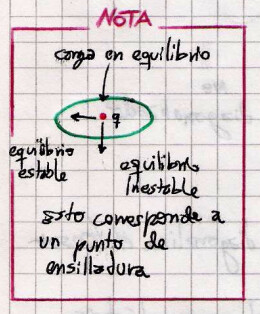
\includegraphics[width=0.32\textwidth]{images/fig_ft1_energiaPic.jpg}}

% =================================================================================================
\section{Esfera con magnetización uniforme}
% =================================================================================================
\[
	\vb{M} = M_0 \hat{z} \qquad \divem{M}= 0 = \rotorm{M}
\]
usando el $\phi_m$ se llega a
\[
	\vb{H}_I = -\frac{4\pi}{3}\vb{M} \qquad \vb{B}_I = \frac{8\pi}{3}\vb{M}
\]
donde $I$ es por interior de esfera y afuera el $\phi_m$ es el de un dipolo con 
\[
	\vb{m} = \frac{4\pi}{3}a^3\vb{M}
\]
y esto vale no solo para grandes distancias sino incluso hasta la superficie (no hay multipolos
subsiguientes).

\begin{figure}[htb]
	\begin{center}
	\includegraphics[width=0.6\textwidth]{images/fig_ft1_magnetiz1.pdf}	 
	\end{center}
	\caption{}
\end{figure} 

En las figuras vemos las líneas de \vb{B} que son continuas, no nacen ni mueren, pero las
de \vb{H} nacen y mueren en la superficie, por la $\sigma_M = \vb{M}\cdot\hat{n}$.
\vb{H} es menos intenso que \vb{B} pues
\[
	\vb{H} = \vb{B} - 4\pi \vb{M}
\]
de manera que en el interior \vb{H} y \vb{B} tienen sentidos opuestos.

% =================================================================================================
\section{Histéresis}
% =================================================================================================

Los campos fundamentales son $\vb{E},\vb{B}$, en realidad $\vb{D},\vb{H}$ se introducen para tener
en cuenta en promedio los efectos de $\rho, \vb{J}$ de las cargas y corrientes atómicas.

Para medios magnéticos (diamagnéticos o paramagnéticos) hay relación lineal
\[
	\vb{B} = \mu \vb{H}
\]
pero para ferromagnéticos es $\vb{B} = f(\vb{H})$ con $f$ no lineal. Se verifica un fenómeno
de histéresis; \vb{B} es una función multivaluada de \vb{H} y $f$ depende de la historia del material.

\begin{figure}[htb]
	\begin{center}
	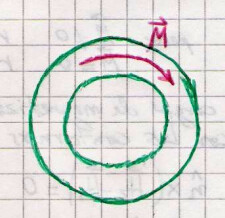
\includegraphics[width=0.6\textwidth]{images/fig_ft1_magnetiz3.pdf}	 
	\end{center}
	\caption{}
\end{figure} 

\vb{H} se conoce como campo desmagnetizante.


% =================================================================================================
\section{Esfera ferromagnética en campo externo}
% =================================================================================================

Si sumergimos la esfera en un $\vb{B}_0$ uniforme tendremos
\[
	\vb{H}_I = \vb{B}_0 - \frac{4\pi}{3} \vb{M} \qquad \vb{B}_I = \vb{B}_0 + \frac{8\pi}{3} \vb{M}
\]
y podemos eliminar \vb{M} de manera que 
\[
	2\vb{H}_I + \vb{B}_I = 3\vb{B}_0
\]

\begin{figure}[htb]
	\begin{center}
	\includegraphics[width=0.6\textwidth]{images/fig_ft1_magnetiz2.pdf}	 
	\end{center}
	\caption{}
\end{figure} 

Vemos en la figura en P el punto de trabajo del imán esférico. Subimos $\vb{B}_0$ hasta saturar la
esfera y luego cuando $\vb{B}_0 = 0$ nos hallamos en P. Hemos recorrido el camino ABP.

Usando la curva de histéresis relacionamos $\vb{B}_I, \vb{H}_I$ y entonces
\[
	\vb{B}_I = 3 \vb{B}_0  - 2 \vb{H}_I.
\]

Un imán es tanto más estable cuando $\vb{H}_I$ es pequeño; en el caso de $\vb{M} \parallel$ superficie,
por ejemplo.

% \bibliographystyle{CBFT-apa-good}	% (uses file "apa-good.bst")
% \bibliography{CBFT.Referencias} % La base de datos bibliográfica

\end{document}
